\documentclass[a4paper, 10pt, titlepage]{report} 

\usepackage{hyperref}
\usepackage[utf8]{inputenc}
\usepackage[spanish]{babel}
\usepackage{mathtools}
\usepackage{graphicx}

% CODE C
\usepackage{amssymb}
\usepackage{listings}
\usepackage{verbatim}
\usepackage{xcolor}
\definecolor{textblue}{rgb}{.2,.2,.7}
\definecolor{textred}{rgb}{0.54,0,0}
\definecolor{textgreen}{rgb}{0,0.0,0}
\lstset{language=C, 
numbers=left, 
numberstyle=\tiny, 
stepnumber=1,
numbersep=5pt, 
tabsize=4,
basicstyle=\ttfamily,
keywordstyle=\color{textblue},
commentstyle=\color{textred},   
stringstyle=\color{textgreen},
frame=none,                    
columns=fullflexible,
keepspaces=true,
xleftmargin=\parindent,
showstringspaces=false}

\title{Iniciación en GNU}
\author{Alberto Fraile}
\date{2020}

\begin{document}

\maketitle
\tableofcontents
\newpage

\chapter*{Introducción}
\addcontentsline{toc}{chapter}{Introducción}
\chapter{Terminal GNU-Linux}
\section{Navegar por los directorios} 
\begin{verbatim}
pwd
\end{verbatim}
<<Muestra la ruta en la que nos encontramos actualmente>>

\begin{verbatim}
ls  //  ls - l
\end{verbatim}
<<Lista el contenido de un directorio // Información adicional>>  

\begin{verbatim}
ls -a
\end{verbatim}
<<Lista el contenido de un directorio, incluidos archivos ocultos>>

\begin{verbatim}
cd // cd ..
\end{verbatim}
<<Nos lleva al directorio raiz // Subimos un nivel>> \


\section{Examinar archivos} 

\begin{verbatim}
file
\end{verbatim}
<<Determina el tipo de un archivo>>

\begin{verbatim}
cat
\end{verbatim}
<<Muestra el contenido de un archivo>>

\begin{verbatim}
less
\end{verbatim}
<<Muestra el contenido de un archivo y lo pagina>> \

\newpage

\section{Manipulación de archivos y directorios}

\begin{verbatim}
mkdir
\end{verbatim}    
<<Crear un directorio>>


\begin{verbatim}
rmdir
\end{verbatim}
<<Elimina un directorio vacio>>

\begin{verbatim}
cp
\end{verbatim}
<<Copia un fichero o directorio>>

\begin{verbatim}
cp -r
\end{verbatim}
<<Copia un directorio con todo su contenido>>

\begin{verbatim}
mv
\end{verbatim}
<<Mueve o renombra un fichero>>

\section{Información del sistema}
\section{Administración}
\section{Procesos}
\section{Permisos}
\section{Actualización}
\section{Inicio y apagado}
\section{Comandos de red}
\section{Comandos de comandos}
\chapter{Composición de textos. \LaTeX}
\section{Elementos y opciones de un documento}

 \begin{verbatim}   


 letterpaper
 a4paper
 a5paper
 b5paper
 legalpaper
 executivepape

 landscape

 10pt
 11pt
 12pt

 oneside
 twoside

 titlepage
 notitlepage

 openright
 openany
 
 onecolumn
 twocolumn
\end{verbatim}   

\newpage

\section{Paquetes comunes}

\begin{verbatim}

\usepackage[<opciones>]{<paquete>}



\end{verbatim}

\newpage

\section{Comandos comunes}

\newpage

\section{La portada del documento}

\newpage

\section{Creación y edición de tablas}

\newpage

\begin{section}{Estructura y desarrollo de un artículo}\end{section}

\begin{lstlisting}
    \documentclass[a4paper, 10pt, titlepage]{article}

    \usepackage{hyperref}
    \usepackage[utf8]{inputenc}
    \usepackage[spanish]{babel}
    \usepackage{graphicx}
    
    \title{Ejemplo}
    \author{Ejempla Ejemplez}
    \date{2020}
    

    \begin{document}

    \maketitle
    \tableofcontents
    
    \\ Nuevo parrafo

    \section{Nombre} 
    \section*{Sin Numeracion}

    \subsection{Nombre} 
    \subsection*{Sin Numeracion}

    \subsubsection{Nombre}

    \textbf{Negrita} \textit{Cursiva} \underline{Subrayado}
    
    \label{'Etiqueta'}
    \ref{'Etiqueta'}

    \begin{quote}
        \small <<Ejemplo de cita>>
    \end{quote}

    \begin{figure}[htp]
        \centering
        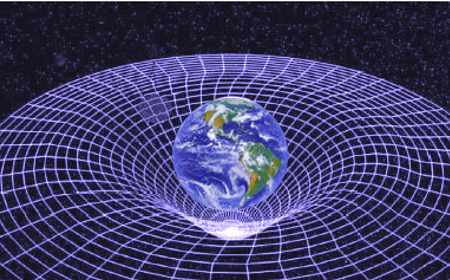
\includegraphics[width=0.8\textwidth]{imagen.jpeg}
        \caption{Descripcion de la fotografia}
        \label{imagenejemplo}
    \end{figure}

    \end{document}
\end{lstlisting}    

\newpage

\begin{section}{Estructura y desarrollo de un libro}\end{section}
   
    \begin{lstlisting}
        \documentclass[a4paper, 10pt, titlepage]{book}
    
        \usepackage{hyperref}
        \usepackage[utf8]{inputenc}
        \usepackage[spanish]{babel}
        \usepackage{graphicx}
        
        \title{Ejemplo}
        \author{Ejempla Ejemplez}
        \date{2020}
        
    
        \begin{document}
    
        \maketitle
        \tableofcontents
        
        \\ Nuevo parrafo
    
        \chapter{Nombre} 
        \chapter*{Sin Numeracion}
    
        \section{Nombre} 
        \section*{Sin Numeracion}
    
        \label{'Etiqueta'}
        \ref{'Etiqueta'}
    
        \begin{quote}
            \small <<Ejemplo de cita>>
        \end{quote}

        \begin{figure}[htp]
            \centering
            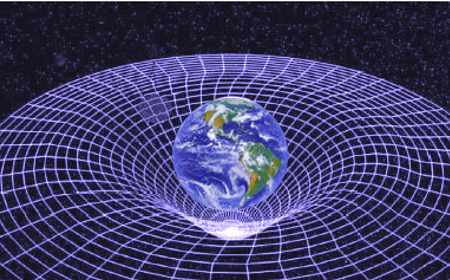
\includegraphics[width=0.8\textwidth]{imagen.jpeg}
            \caption{Descripcion de la fotografia}
            \label{imagenejemplo}
        \end{figure}

        \end{document} \end{lstlisting} \hfill
        
        
        \small  <<Numeración a los costados. Los capítulos comienzan siempre en página impar.>>

\newpage

\section{Estructura y desarrollo de un reporte}

\begin{lstlisting}
    \documentclass[a4paper, 10pt, titlepage]{report}

    \usepackage{hyperref}
    \usepackage[utf8]{inputenc}
    \usepackage[spanish]{babel}
    \usepackage{graphicx}
    
    \title{Ejemplo}
    \author{Ejempla Ejemplez}
    \date{2020}
    

    \begin{document}

    \maketitle
    \tableofcontents
    
    \\ Nuevo parrafo

    \chapter{Nombre} 
    \chapter*{Sin Numeracion}

    \section{Nombre} 
    \section*{Sin Numeracion}

    \label{'Etiqueta'}
    \ref{'Etiqueta'}

    \begin{quote}
        \small <<Ejemplo de cita>>
    \end{quote}

    \begin{figure}[htp]
        \centering
        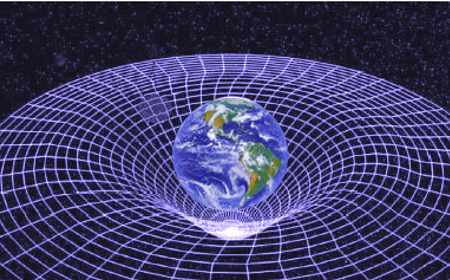
\includegraphics[width=0.8\textwidth]{imagen.jpeg}
        \caption{Descripcion de la fotografia}
        \label{imagenejemplo}
    \end{figure}

    \end{document}\end{lstlisting}      
    
    \small<<Los capítulos comienzan en página siguiente a la finalización del anterior .>>

\newpage 

\section{Estructura y desarrollo de una carta}

\begin{lstlisting}

    \documentclass{letter}
    \usepackage{hyperref}
    \signature{Marcelo Bielsa}
    \address{Anfield Road 58 \\ Leeds \\ 58100 Leeds}
    \begin{document}
    
    \begin{letter}{Director \\ Diario el Pais \\ Avenida de la Constitucion 10
    \\ Sevilla \\ 41000 Sevilla}
    \opening{Estimado Sr. Director:}
    
    Cuerpo de la carta
    
    \closing{Atentamente,}
    
    \ps
    
    P.S. Posdata
    
    \end{letter}
    \end{document}    

\end{lstlisting}
    
\newpage


\chapter{Bases de datos. Mariadb}
\section{Acceso a Mariadb}

\begin{verbatim}
sudo mariadb -u root -p 
\end{verbatim}

\section{Creación y acceso a la base de datos} 

\begin{verbatim}
CREATE DATABASE Ejemplo;
\end{verbatim}
<<Crear nueva base de datos>> 
\begin{verbatim}
SHOW DATABASES; 
\end{verbatim}
<<Visualizar las bases de datos existentes>> 
\begin{verbatim}
USE Ejemplo; 
\end{verbatim}
<<Acceder a la base de datos seleccionada>> \\

\section{Creación y modificación de tablas}

\begin{verbatim}
CREATE TABLE Ejemplo ( 
ID int(10) not null, auto_increment,
Nombre varchar(20) not null,
Apellido varchar(20) not null,
PRIMARY KEY (ID) );
\end{verbatim}
<<Creación de tabla en la base de datos>> 
\begin{verbatim}
SHOW TABLES Ejemplo; 
\end{verbatim}
<<Visualizar tablas de la base de datos>> 
\begin{verbatim}
DESCRIBE Ejemplo;
\end{verbatim}
<<Muestra los campos contenidos en una tabla>> 
\begin{verbatim}
RENAME TABLE Ejemplo \textbf{TO} Personas;
\end{verbatim}
<<Renombrar tabla>>
\begin{verbatim}
ALTER TABLE Ejemplo ADD id int(10), not null, auto_increment;
\end{verbatim}
<<Añadir nuevo campo a la tabla>> 
\begin{verbatim}
ALTER TABLE Ejemplo CHANGE id ID;
\end{verbatim}
<<Cambiar nombre de la tabla>> \\
\begin{verbatim}
ALTER TABLE Ejemplo CHANGE Nombre Nombre VARCHAR(20);
\end{verbatim}
<<Cambiar tipo de dato de la tabla>> 
\begin{verbatim}
DROP TABLE Personas;
\end{verbatim}
<<Eliminar tabla>> 
\begin{verbatim}
DELETE FROM Ejemplo WHERE Edad =10;
\end{verbatim}
<<Eliminar registros de una tabla segun condiciones>> 
\begin{verbatim}
UPDATE Ejemplo SET Nombre, Edad WHERE ID =1;
\end{verbatim}
<<Actualizar registros de la tabla>> 
\begin{verbatim}
BACKUP DATABASE Ejemplo TO DISK = Ubicacion;
\end{verbatim}
<<Backup de la base de datos>> 
\begin{verbatim}
BACKUP DATABASE Ejemplo TO DISK = Ubicacion WITH DIFFERENTIAL;
\end{verbatim}
<<Backup de las partes cambiadas desde la ultima vez>> 
\begin{verbatim}
INSERT INTO Ejemplo
(ID, Nombre, Apellido, Edad)
VALUES
(1, Alberto, Hernandez, 40),
(2, Javier, Sevilla, 45),
(3, Alfredo, Martinez, 65);
\end{verbatim}
<<Insertar múltiples registros en una tabla>>

\section{Consultas}
\begin{verbatim}
SELECT * FROM Ejemplo;
\end{verbatim}
<<Consultar todo el contenido de la tabla>> 
\begin{verbatim}
SELECT ID, Nombre FROM Ejemplo; 
\end{verbatim}
<<Consultar el contenido de la tabla por columnas>> 
\begin{verbatim}
SELECT ID, Nombre FROM Ejemplo WHERE Edad = 40;
\end{verbatim}
<<Consultar el contenido por columnas de la tabla con condiciones>> 
\begin{verbatim}
SELECT Nombre FROM Ejemplo WHERE Edad = 40 AND Nombre = Alberto; 
\end{verbatim}
<<Conultar el contenido con mas de una condicion>> 
\begin{verbatim}
SELECT * FROM Ejemplo WHERE Nombre IS NOT NULL / IS NULL;
\end{verbatim}
<<Comprobar si hay resistros vacios en los distintos campos de la tabla>> 
\begin{verbatim}
 SELECT * FROM Ejemplo ORDER BY Estatura;
\end{verbatim}
 <<Consultar el contenido de la tabla ordenado por parametros>> 
\begin{verbatim}
 SELECT * FROM Ejemplo ORDER BY Estatura DESC;
\end{verbatim}
 <<Consultar el contenido de la tabla por orden descendente>> 
\begin{verbatim}
 SELECT * FROM Ejemplo ORDER BY Estatura ASC;
\end{verbatim}
 <<Consultar el contenido de la tabla por orden ascendente>> 
 \begin{verbatim}
 SELECT * FROM Ejemplo ORDER BY Estatura DESC, Peso ASC; \end{verbatim}
 <<Consultar el contenido de la tabla con distintos parámetros y órdenes>> 
 \begin{verbatim}
 SELECT TOP 4 FROM Ejemplo;
\end{verbatim}
 <<Devuelve un numero determinado de registros>> 
\begin{verbatim} 
SELECT MAX(Ejemplares) FROM Ejemplo WHERE ID =1;
\end{verbatim}
<<Devuelve el valor máximo de una columna>> 
\begin{verbatim}
SELECT MIN(Ejemplares) FROM Ejemplo WHERE ID =1;
\end{verbatim}
<<Devuelve el valor mínimo de una columna>> 
\begin{verbatim}
SELECT COUNT(Ejemplares) FROM Ejemplo WHERE ID =1;
\end{verbatim}
<<Devuelve el numero de filas que coinciden con las condicione>> 
\begin{verbatim}
SELECT AVG(Ejemplares) FROM Ejemplo WHERE ID =1;
\end{verbatim}
<<Devuelve el valor promedio de una columna>> 
\begin{verbatim}
SELECT SUM(Ejemplares) FROM Ejemplo WHERE ID =1;
\end{verbatim}
<<Devuelve la suma de una columna numerica>> 
\begin{verbatim}
SELECT * FROM Ejemplo WHERE Nombre LIKE "a%";
\end{verbatim}
<<Muestra las personas cuyo nombre empieza por a>> 
\begin{verbatim}
SELECT * FROM Ejemplo WHERE Nombre LIKE "%a";
\end{verbatim}
<<Muestra las personas cuyo nombre acaba por a>> 
\begin{verbatim}
SELECT * FROM Ejemplo WHERE Nombre LIKE "%a%";
\end{verbatim}
<<Muestra las personas cuyo nombre contenga una a>> 
\begin{verbatim}
SELECT * FROM Ejemplo WHERE Nombre LIKE "_a%";
\end{verbatim}
<<Muestra las personas cuyo nombre contenga una a en segunda posicion>> 
\begin{verbatim}
SELECT * FROM Ejemplo WHERE nombre LIKE "a__%";
\end{verbatim}    
<<Muestra personas cuyo nombre empieza por a y tiene al menos 3 letras>>

\newpage

\begin{verbatim}
SELECT * FROM Ejemplo WHERE nombre LIKE "[abc]%";
\end{verbatim}
<<Muestra las personas cuyo nombre empieza por a, b o c>>
\begin{verbatim}
SELECT * FROM Ejemplo WHERE nombre LIKE "[!abc]%";
\end{verbatim}
<<Muestra las personas cuyo nombre no empieza por a, b o c>>
\begin{verbatim}
SELECT * FROM Ejemplo WHERE nombre NOT LIKE "[abc]%";
\end{verbatim}
<<Muestra las personas cuyo nombre no empieza por a, b o c>>
\begin{verbatim}
SELECT * FROM Ejemplo WHERE pais IN ('Espana', 'Cuba');
\end{verbatim}
<<Muestra las personas que estan en España o Cuba>>
\begin{verbatim}
SELECT * FROM Ejemplo WHERE pais NOT IN ('Espana', 'Cuba');
\end{verbatim}
<<Muestra las personas que no estan en España o Cuba>>
\begin{verbatim}
SELECT * FROM Ejemplo WHERE pais IN (SELECT pais FROM Ciudades);
\end{verbatim}
<<Muestra las personas que estan en los mismos paises que las ciudades>>
\begin{verbatim}
SELECT * FROM Ejemplo WHERE estatura BETWEEN 100 AND 200;
\end{verbatim}
<<Muestra las personas cuya estatura esta entre 100 y 200>>
\begin{verbatim}
SELECT * FROM Ejemplo WHERE estatura NOT BETWEEN 100 AND 200;
\end{verbatim}
<<Muestra las personas cuya estatura no esta entre 100 y 200>>
\begin{verbatim}
SELECT * FROM Ejemplo WHERE estatura BETWEEN 100 AND 200 
AND id NOT IN (1, 2);
\end{verbatim}
<<Muestra personas de estatura entre 100-200 y no las cuyo id es...>>
\begin{verbatim}
SELECT * FROM Ejemplo WHERE nombre BETWEEN "Alberto" 
AND "Manuel" ORDER BY nombre;
\end{verbatim}
<<Muestra las personas entre Alberto y Manuel ordenado por nombre>>
\begin{verbatim}
SELECT * FROM Ejemplo WHERE nombre NOT BETWEEN "Alberto" 
AND "Manuel" ORDER BY nombre;
\end{verbatim}
<<Muestra las personas que no estan entre Alberto y Manuel ordenado por nombre>>
\begin{verbatim}
SELECT * FROM Ejemplo WHERE FNac BETWEEN #01/07/20# AND #31/07/20#;
\end{verbatim}
<<Muestra las personas cuya fecha de nacimiento esta entre...>>
\begin{verbatim}
SELECT Idpersona AS Id, edad AS Ed FROM Ejemplo;   
\end{verbatim}
<<Crear alias para las columnas idpersona y edad>>

\newpage

\section{Relaciones 0:N - 1:N (Uno a muchos)}

\begin{verbatim}
ALTER TABLE Ejemplo ADD  (
Ordenador int(5) not null,
FOREIGN KEY(Ordenador) REFERENCES Ordenadores(IdPc)  );
\end{verbatim}
<<Creación del campo que relacciona los parámetros con clave secundaria>>
\begin{verbatim}
SELECT * 
FROM Ejemplo ej, Persona_Telefono pt, Telefonos t 
WHERE ej.Idpersonal = pt.Idpersonas AND t.Idtelefono 
= pt.Idtelefono;  
\end{verbatim}
<<.....>>
\begin{verbatim}
SELECT * 
FROM Ejemplo ej 
JOIN Persona_Telefono ejt ON p.Idpersonal = ejt.Idpersonas 
JOIN Telefonos t ON pt.Idtelefono = t.Idtelefono;  
\end{verbatim}
<<.....>>


\section{Relaciones N:M (muchos a muchos)}

*** PENDIENTE ***

\chapter{Programación. Python}
\section{Comandos básicos}
\chapter{Scripts}
\chapter{Redes}
\chapter{Seguridad informática}
\section{Navegador web}
\chapter{Cifrado}
\section{Criptografía. Técnicas de cifrado}
\section{El protocolo SSH}
\chapter{Raspberry Pi}
\section{Hardware. Características y posibilidades}
\section{Proyectos}
\subsection{Cluster}


\end{document}